% \pagebreak[4]
% \hspace*{0.5cm}
% \pagebreak[4]
% \hspace*{1cm}
% \pagebreak[4]

\chapter{Tổng Quan}
\ifpdf
    \graphicspath{{Chapter1/Chapter1Figs/PNG/}{Chapter1/Chapter1Figs/PDF/}{Chapter1/Chapter1Figs/}}
\else
    \graphicspath{{Chapter1/Chapter1Figs/EPS/}{Chapter1/Chapter1Figs/}}
\fi

\section{Giới thiệu đề tài}
\markboth{\MakeUppercase{\thechapter. Tổng Quan }}{\thechapter. Tổng Quan}
Với việc khánh thành phòng học thông minh, một không gian học mở dành cho sinh viên UIT với các trang thiết bị tiên tiến. Tuy nhiên, đi cùng với việc chất lượng giảng dạy được nâng cao, nhu cầu bảo vệ tài sản công đã trở thành một vấn đề cực kỳ quan trọng và được đặt lên hàng đầu. Để đảm bảo an ninh và tránh mất tài sản công, nhóm nghiên cứu đã quyết định thực hiện đề tài “Hệ thống phát hiện các thiết bị trong phòng học thông minh thời gian thực”. 

Bài toán nghiên cứu có đầu vào là hình ảnh (image) được trích xuất từ 2 camera giám sát thuộc phòng học thông minh của trường, đầu ra là hình ảnh (image) đã được xử lý để phát hiện các trang thiết bị (màn hình, chuột, bàn phím) trong thời gian thực. Đây là bài toán có tính cấp thiết và ứng dụng cao, với mục đích đặt ra nhằm bảo vệ tài sản công của nhà Trường, tránh việc thiệt hại về các trang thiết bị. Ngoài ra, đề tài còn có thể mở rộng ứng dụng trong nhiều địa điểm thuộc nhà Trường, hay phạm vi bên ngoài nhà Trường. 

\begin{figure}[h!]
	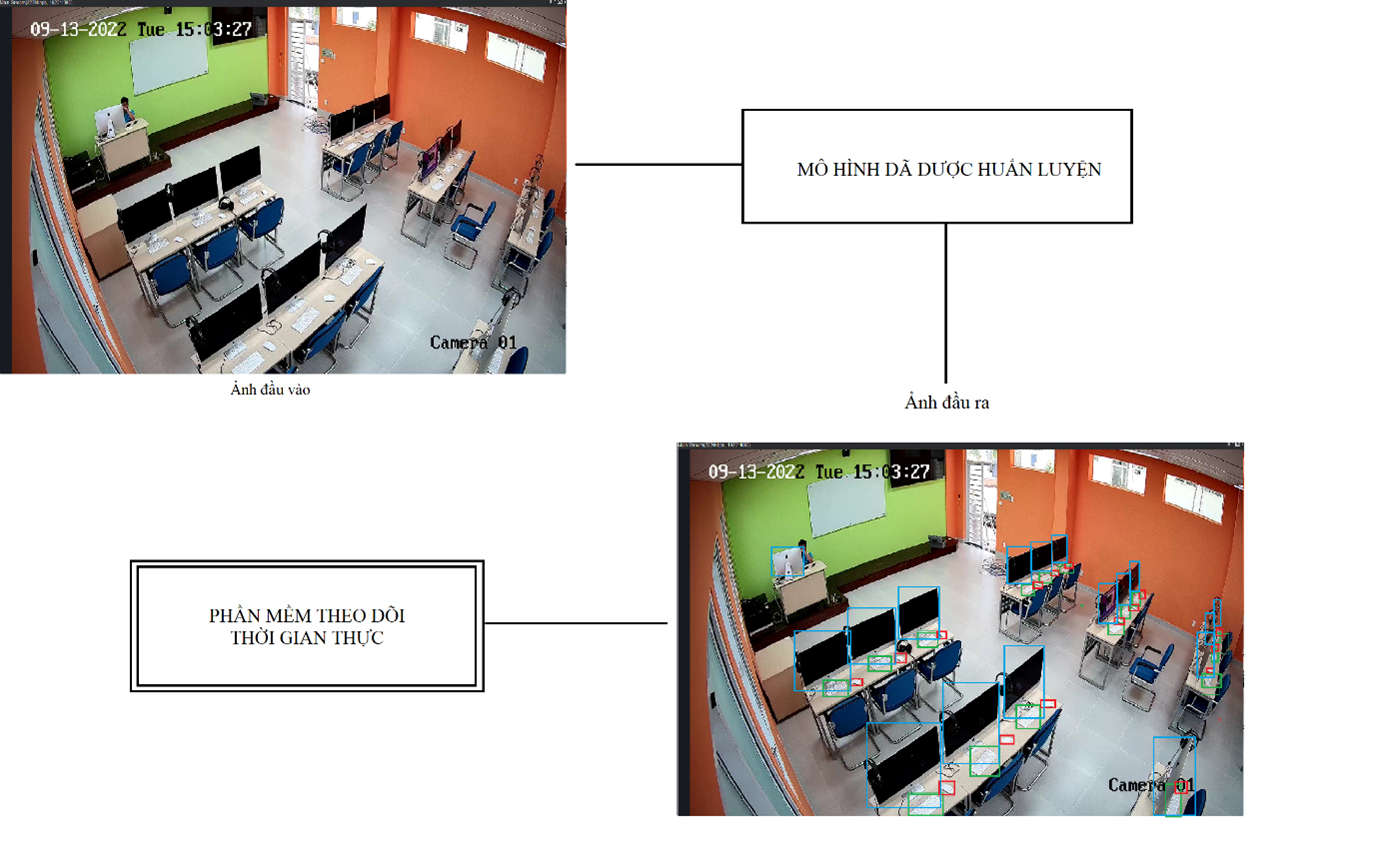
\includegraphics[scale=1]{tong-quan-bai-toan.png}
	\caption{Các bước xử lý cơ bản của hệ thống}
\end{figure}

	Tuy nhiên, bài toán phát hiện các thiết bị trong phòng học thông minh không phải là một bài toán đơn giản. Với yêu cầu phát hiện các thiết bị trong thời gian thực, đòi hỏi hệ thống phải có khả năng phát hiện các thiết bị một cách nhanh chóng và chính xác, từ đó giúp người quản lý phòng học có thể có những biện pháp kịp thời để bảo vệ tài sản công. Đề tài nghiên cứu còn gặp phải vấn đề khoảng cách từ 2 camera giám sát được đặt ở trên cao, dẫn đến việc khoảng cách đến các thiết bị có thể khác nhau, khiến hình ảnh của chúng bị mờ hay có thể bị che khuất bởi các thiết bị khác. Bên cạnh đó, việc sử dụng 2 camera giám sát làm tăng thêm tầm nhìn nhưng lại phát sinh thêm bài toán phải đồng bộ giữa chúng để tránh nhận diện một thiết bị đến 2 lần. Không những thế, phòng học thông minh chỉ vừa được khánh thành cách đây không quá lâu, nên bài toán còn chịu sự hạn chế về mặt dữ liệu.   
	
	Hiện nay, có khá nhiều phương pháp đối với bài toán phát hiện vật thể nhưng chưa thực sự áp dụng cho một lĩnh vực cụ thể như đề tài, nên việc lựa chọn phương pháp phù hợp và tối ưu nhất cho đề tài nghiên cứu cũng là một thách thức lớn.


\section{Tính cấp thiết}
\markboth{\MakeUppercase{\thechapter. Tổng Quan }}{\thechapter. Tổng Quan}
Đề tài nghiên cứu khoa học này là cấp thiết vì những đặc điểm sau:
\begin{enumerate}
	\itemsep0em 
	\item Tính ứng dụng cao: Hỗ trợ bảo vệ trang thiết bị của nhà Trường, tránh những mất mát xuất phát từ ý thức của một số thành viên trong quá trình sử dụng tài sản công.
	\item Thiếu hụt trong nghiên cứu trước đây: Mặc dù đã có nghiên cứu về nhận diện vật thể, tuy nhiên, vẫn chưa có bất kỳ mô hình nào để bảo vệ cụ thể các trang thiết bị trong phòng máy (máy tính, chuột, bàn phím). Điều này cho thấy sự cấp thiết của đề tài này để giải quyết vấn đề thiếu hụt này.
	\item Thiếu ứng dụng minh họa: Hiện tại chưa có ứng dụng minh họa nào cho đề tài này. Việc tạo ra một ứng dụng minh họa sẽ giúp cho người sử dụng dễ dàng hiểu được cách thức hoạt động của hệ thống bảo vệ trang thiết bị.
\end{enumerate}

Tóm lại, đề tài nghiên cứu khoa học này cấp thiết vì nó giúp bảo vệ trang thiết bị của nhà trường, giải quyết thiếu hụt trong nghiên cứu trước đây và cần có ứng dụng minh họa để giúp người dùng dễ dàng hiểu được hệ thống bảo vệ trang thiết bị.


\section{Thách thức}
\markboth{\MakeUppercase{\thechapter. Tổng Quan }}{\thechapter. Tổng Quan}
Đề tài phải đối diện với một số thách thức đáng kể, bao gồm:

\begin{enumerate}
	\itemsep0em 
	\item Xây dựng hệ thống trong thời gian thực yêu cầu cả sự suy diễn nhanh chóng trong khi vẫn duy trì được độ chính xác gốc của mô hình.
	\item Vấn đề đồng bộ hóa giữa 2 camera do khác biệt về vị trí đặt và khoảng cách đến các thiết bị.
	\item Dữ liệu đầu vào vẫn còn hạn chế về số lượng lẫn chất lượng.
\end{enumerate}


\section{Ý tưởng khoa học}
\markboth{\MakeUppercase{\thechapter. Tổng Quan }}{\thechapter. Tổng Quan}
Trong lĩnh vực Computer Vision, bài toán nhận diện vật thể đóng vai trò rất quan trọng và đang nhận được nhiều sự quan tâm. Các mô hình nhận diện vật thể đang được nghiên cứu và phát triển liên tục để có thể đáp ứng được nhu cầu xã hội.

Hiện nay, các mô hình nhận diện vật thể thường được các nhóm nghiên cứu tiếp cận thông qua thuật toán YOLO – một state-of-the-art trong lĩnh vực Computer Vision, cụ thể hơn là bài toán nhận diện vật thể (Object detection). Tuy nhiên, bên cạnh YOLO, vẫn còn một hướng tiếp cận phổ biến thông qua các thuật toán two-stages, sử dụng mạng neural tích chập, mà tiêu biểu của trong số đó là Faster R-CNN. Do đó, việc tìm hiểu và đánh giá các phương pháp tiếp cận đóng vai trò rất lớn trong việc xây dựng hệ thống.


\section{Mục tiêu hướng tới}
\markboth{\MakeUppercase{\thechapter. Tổng Quan }}{\thechapter. Tổng Quan}
Trong công trình nghiên cứu này, các mục tiêu đề ra bao gồm:

\begin{enumerate}
	\itemsep0em 
	\item Tìm hiểu tổng quan về bài toán nhận diện vật thể (object detection).
	\item Đánh giá một số phương pháp tiên tiến có thể giải quyết đề tài nhận diện các thiết bị trong phòng học thông minh.
	\item Xây dựng tập dữ liệu cho đề tài và đánh giá các phương pháp đã tìm hiểu trên tập dữ liệu đó.  
	\item Sử dụng phương pháp đã thực hiện để xây dựng ứng dụng minh họa.
\end{enumerate}

Theo đó, phạm vi nghiên cứu của đề tài như sau:
\begin{enumerate}
	\itemsep0em 
	\item Đánh giá một số phương pháp:
	\begin{itemize}
		\itemsep0em 
		\item Thuật toán Two-stages mà tiêu biểu là Faster R-CNN.
		\item Thuật toán One-stage với YOLOv7.
	\end{itemize}
	\item Xây dựng tập dữ liệu: Thu thập dữ liệu qua 2 camera giám sát thuộc phòng học thông minh. 
\end{enumerate}

%\begin{figure}[!htbp]
%  \begin{center}
%    \leavevmode
%    \ifpdf
%      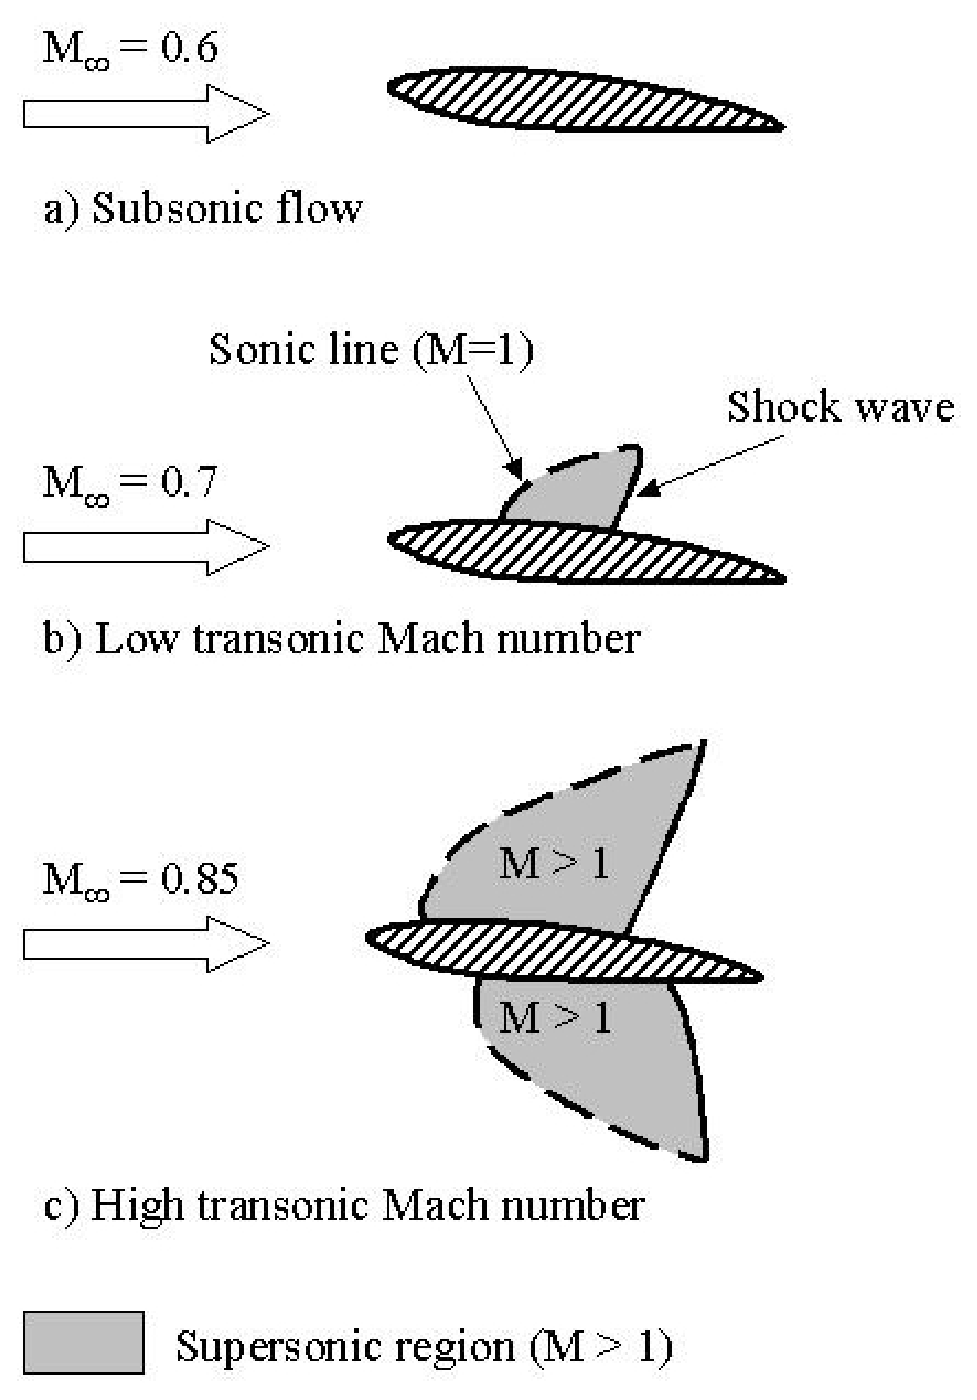
\includegraphics[height=6in]{aflow}
%    \else
%      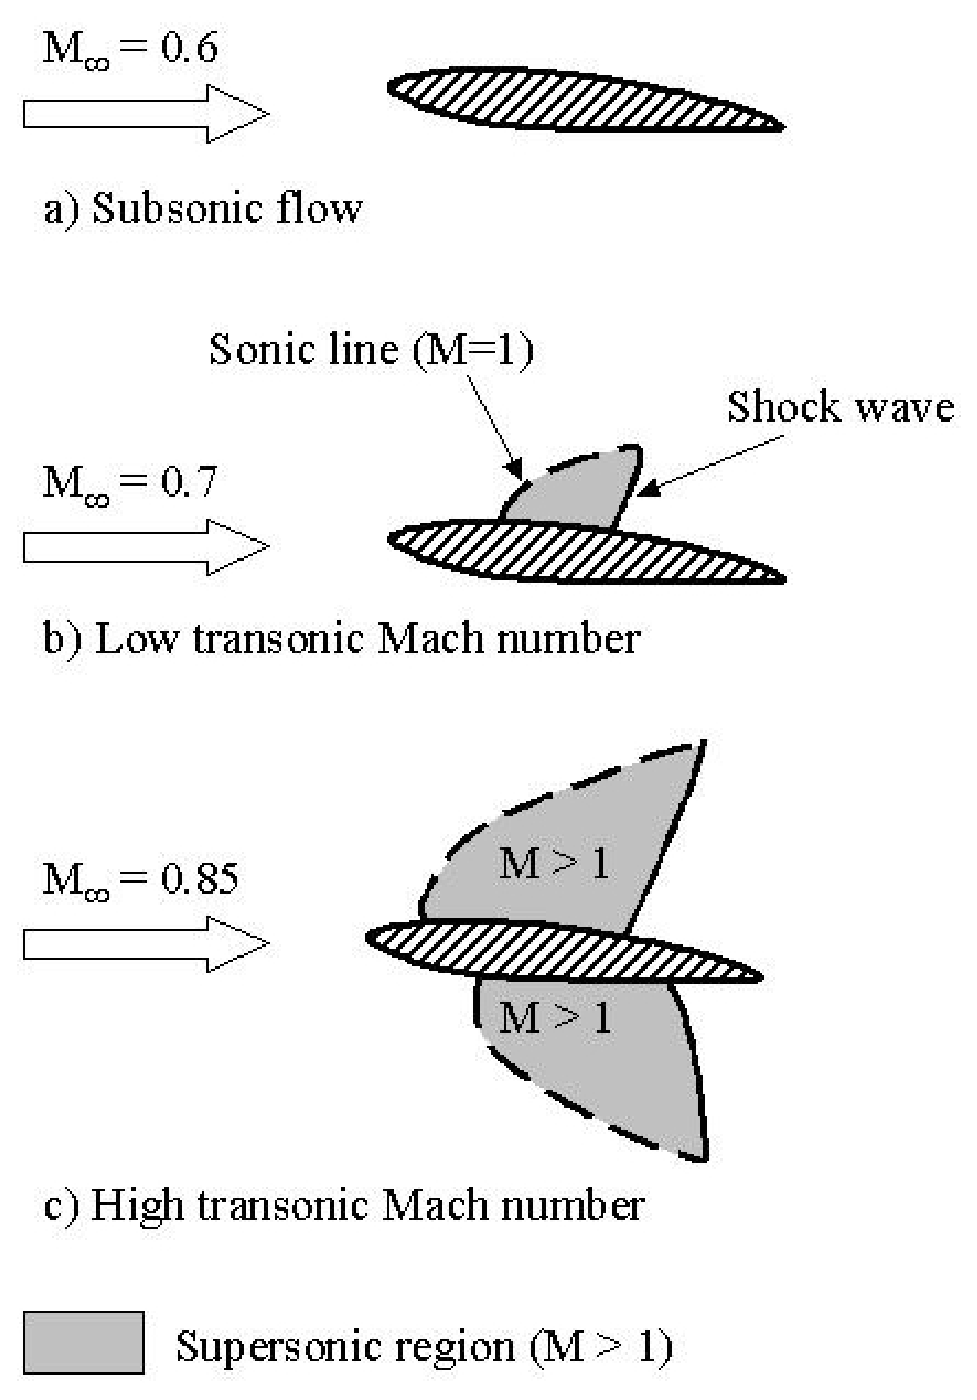
\includegraphics[bb = 92 86 545 742, height=6in]{aflow}
%    \fi
%    \caption{Airfoil Picture}
%    \label{FigAir}
%  \end{center}
%\end{figure}

% above code has been macro-fied in Classes/MacroFile.tex file
%\InsertFig{\IncludeGraphicsH{aflow}{6in}{92 86 545 742}}{Airfoil Picture}{FigAir} 
